\documentclass[%
 reprint,
 superscriptaddress,
 amsmath,amssymb,
 nofootinbib,
 prd,
]{revtex4-2}

\usepackage{graphicx}
\usepackage{dcolumn}
\usepackage{bm}
\usepackage{tensor}
\usepackage{amsmath}
\usepackage{mathrsfs}
\usepackage{amsthm,amsfonts,amssymb}
\usepackage{aas_macros}
\usepackage{CJKutf8}
\usepackage{orcidlink}
\usepackage{soul}

\makeatletter
\newcommand{\refjnl}[1]{{\rmfamily#1}}
\makeatother

\newcommand{\vdag}{(v)^\dagger}
\newcommand\aastex{AAS\TeX}
\newcommand\latex{La\TeX}

\newcommand{\red}{\textcolor{red}}
\newcommand{\AddCite}{\red{[Needs citation]}}
\newcommand{\hyw}[1]{{\color{red}{[{#1}]}}}
\newcommand{\hywcom}[1]{{\color{purple}{[HYW: #1]}}}

\usepackage{fix-cm}
\usepackage{amsmath}
\usepackage{soul}
\usepackage{hyperref}
\usepackage{CJKutf8}
\usepackage{appendix}
\usepackage{xcolor}
\usepackage{graphicx}
\usepackage{duckuments}
\usepackage{tikzducks}
\usepackage{orcidlink}


\begin{document}
\begin{CJK*}{UTF8}{gbsn}
\title{Towards Multiscale Neural Operator Framework of Accretion and Feedback Applications}

\author{Nihaal Bhojwani $^\delta$}
\affiliation{Computing and Mathematical Sciences, California Institute of Technology, CA 91125, USA}
\affiliation{Department of Computer Sciences, University of Maryland}

\author{Chuwei Wang (王楚惟) $^\delta$ \orcidlink{0009-0008-1252-0114}}
\affiliation{Computing and Mathematical Sciences, California Institute of Technology, CA 91125, USA}

\author{Hai-Yang Wang (王海洋) $^\delta$ \orcidlink{0000-0001-7167-6110}} 
\affiliation{TAPIR, California Institute of Technology, Pasadena, CA 91125, USA}
\affiliation{Walter Burke Institute for Theoretical Physics, California Institute of Technology, Pasadena, CA 91125, USA}

\author{Chang Sun (孙畅) \orcidlink{0000-0003-2774-175X}}
\affiliation{Department of Physics, California Institute of Technology, Pasadena, CA 91125, USA}

\author{Elias R. Most \orcidlink{0000-0002-0491-1210}}
\affiliation{TAPIR, California Institute of Technology, Pasadena, CA 91125, USA}
\affiliation{Walter Burke Institute for Theoretical Physics, California Institute of Technology, Pasadena, CA 91125, USA}

\author{Anima  Anandkumar \orcidlink{0000-0002-6974-6797}}
\affiliation{Computing and Mathematical Sciences, California Institute of Technology, CA 91125, USA}


\begin{abstract}
% Black hole feedback zoom-in and out \cite{Guo:2025sjb}
We present the method combining neural operator (NO) and direct \hyw{multi-level} numerical simulations for accretion and feedback problem, in both magnetohydrodynamic (MHD) and general relativistic magnetohydrodynamic (GRMHD) simulations. 
NO is trained to learn the semigroup of the numerical simulation at small scale and provide the boundary condition for the next level of simulation.
As a first step towards multiscale simulations, we focus on black hole feeding and feedback problem.
\hyw{Findings:}
This method is generally applicable as the subgrid model of all the central accretor problems.
\end{abstract}

\maketitle
\footnotetext{\footnotesize $\delta$ equal contribution}
% \footnote{$\delta$ equal contribution}

\end{CJK*}

\section{Introduction}

\hywcom{Multiscale problems.}
Numerical simulations in astrophysics enables us to investigate a broad range of highly complex problems.
Yet many longstanding questions persist because these systems are intrinsically multiscale in both space and time.
Systems with a central accretor—such as the coevolution of supermassive black holes (SMBH) and their host galaxies, star and planet formation, and stellar-mass black holes or neutron stars in supernova remnants—are canonical examples of such multiscale phenomena.

Among all these multiscale problems, feeding and feedback of the SMBHs attracted a lot of attentions.
The SMBHs harbored at the centers of most galaxy nuclei play a crucial role in the evolution of the galaxies, shown in various properties such as stellar and dark matter bulge masses \AddCite.
Ideally one needs to resolve the small-scale dynamics near the event horizon (mpc size), while simultaneously
resolving the large-scale dynamics of the host galaxy (kpc to Mpc size),
making this a formidable task for direct numerical simulations.
Consequently, the accretion flows around SMBHs and their feedbacks are modelled typically by a subgrid model in cosmological simulation \AddCite. 
And the accretion and outflow dynamics near the black hole are often modeled by general relativistic magnetohydrodynamis simulations (GRMHD).
Due to the ignorance of accretion disk formation history, a torus in hydrodynamic equilibrium is usually adopted as the idealized initial condition \cite{1976ApJ...207..962F}.
Early attempt to bridge the feeding problem and construct a more realistic black hole accretion problem includes modelling infall and accretion from the Bondi radius \cite{Bondi:1952MNRAS.112..195B}.

\hywcom{Relativistic outflows.}
The feedback from low-Eddington accreting black holes are carried out mainly through relativistic outflows (winds and jets) \AddCite.
Especially, the jets are observed from AU to Mpc scales, far beyond the range of host galaxies. 
These relativistic outflows can efficiently deposit energy and momentum into the interstellar medium (ISM) and intergalactic medium (IGM), triggering large-scale turbulence, and thus affect the star formation and galaxy evolution \AddCite.

\hywcom{Black hole feeding and feedback problem.}
\hywcom{And Computational advances.}
A considerable amount of efforts adopting various techniqueshas been made to bridge different scales, 
which includes direct simulation assuming smaller scale separation \cite{Lalakos:2022qhl,Lalakos:2023ean,S:2023gta,Lalakos:2025msz},
``zoom-in'' adopting nested mesh in grid codes \cite{Guo2023,Guo2024}, and ``Lagrangian hyper-refinement'' in Lagrangian codes \cite{Hopkins:2023ipv,Hopkins2023},
remapping between different simulations, 
and ``multi-zone'' \cite{Cho:2023wqr,Cho:2024wsp,Cho:2025lzq} or ``cyclic-zoom'' \cite{Guo:2025sjb} methods iteratively 
refining and de-refining the simulation domain near the central black hole.
Earlier attempts on bridging scales adopting ``two-zone'' techniques have been made in the content of hydrodynamic accretion  \cite{Yuan:2012ApJ...761..129Y}.


\hywcom{Spatial-Temporal multiscale variability problem.}
Except the direct simulation modifying the scale separation, only the ``multi-zone'' and ``cyclic-zoom'' methods are able to capture feedback from the small-scale and evolve the different domains to convergence.
These two methods are very similar, but different in details, particularly the treatment on how to mask the inner levels when simulating the outer domains. 
``Multi-zone''
``Cyclic-zoom'' masked the inner levels by freezing the hydrodynamic variables while evolving the magnetic fields within the mask region using inductive electic fields, presering the divergence-free constraints on smaller scaler through constraint transport \cite{Balsara:1999JCoPh.149..270B,Gardiner2008}.

\hywcom{Temporal variability hierarchy.}
Despite the huge success of these novel methods, they could still suffer from the temporal variability problem.

\hywcom{Neural Operator}
In this paper, we start 

\hywcom{Paper Structure.}
The structure of the paper is as follows. 
\hywcom{multiscal-NO?}
In Section \ref{sec:method-simulation} and \ref{sec:method-no}, we describe the numerical methods for direct simulations and algorithm of NO.
In Section \ref{sec:setup}, we describe the problem setups and datasets used for training NOs.
In Section \ref{sec:results}, we present the results: comparing the long-term roll-out of NOs and the direct simulations, and showing the large-scale simulations with NOs as the inner boundary condition.
We then conclude in Section \ref{sec:conclusion}.


\section{Difficult of Capturing Variability in Multiscale Problems}
\label{sec:variability}
                                                                                                                                 

\section{Overview of Multiscale-NO Framework}
\label{sec:overview}

\subsection{Run Duration}


\section{Method-Simulation}
\label{sec:method-simulation}

We use a performance portable version of \texttt{Athena++}~\cite{Stone2020} based on \texttt{Kokkos} library~\cite{Trott2021}-\texttt{AthenaK}~\cite{athenak}.

\subsection{Magneto-hydrodynamics Simulations: Magnetized SCAF}
The setup we use in this work is a magnetized version of SCAF \cite{Guo2024}, without cooling and heating terms. 
In this case, we solve the Newtonian magnetohydrodynamics equations in conservative form:
\begin{align}
    \frac{\partial \rho}{\partial t}+\nabla \cdot(\rho \boldsymbol{v}) &=s_{\rho}\,, \\
    \frac{\partial(\rho \boldsymbol{v})}{\partial t}+\nabla \cdot(\rho \boldsymbol{v} \boldsymbol{v} + P \boldsymbol{I}  - \boldsymbol{B}\boldsymbol{B})&=\boldsymbol{s_p}-\rho \nabla \Phi\,, \\
    \frac{\partial E}{\partial t}+\nabla \cdot[(E+{P}) \boldsymbol{v} - \left(\boldsymbol{B}\cdot \boldsymbol{v}\right) \boldsymbol{B}]&=s_E-\rho \boldsymbol{v} \cdot \nabla \Phi,\\
    \frac{\partial \boldsymbol{B}}{\partial t}-\nabla \times [ \boldsymbol{v} \times \boldsymbol{B} ]&=0\,,
\end{align}
where $\rho:\mathbb{R}^3\to\mathbb{R}$ is the gas density, $\boldsymbol{v}:\mathbb{R}^3\to\mathbb{R}^3$ is the velocity, $P:\mathbb{R}^3\to\mathbb{R}$ is the pressure, $E=P/(\gamma-1)+\rho |v|^2/2$ is the total energy density, and $-\nabla\Phi$ is the gravitational acceleration due to the central accretor. The flow evolved following ideal gas law with adiabatic index $\gamma=5/3$.

In code unit, $GM=r_0=\rho_0=1$. The output quantities include $(\rho, P, \boldsymbol{v}=(v_x, v_y, v_z), \boldsymbol{B}=(B_x, B_y, B_z))$.

We use piecewise parabolic reconstruction \citep{Colella1984}, an HLLD Riemann solver \citep{Miyoshi2005},  a constraint transport algorithm \citep{Gardiner2008} for the divergence-free magnetic field evolution, and first-order flux correction \cite{2009ApJ...691.1092L}.

\subsection{GRMHD Simulations}
The conservative Valencia formulations for solving GRMHD equations with induction equation
\begin{align}
     &\partial_t\boldsymbol{U} + \partial_i\boldsymbol{F}=\boldsymbol{S} \\
     &\partial_t (\sqrt{-g}B^i)+\partial_j(\sqrt{-g}(b^iu^j-b^ju^i))=0
\end{align}
where the conserved variables, fluxes, and source terms associated with the connection are
\begin{equation}
\begin{aligned}
\mathbf{U} &=\sqrt{-g}\left[\begin{array}{c}
\rho u^t \\
T_i^t \\
T_t^t+\rho u^t
\end{array}\right], \\
\mathbf{F} &=\sqrt{-g}\left[\begin{array}{c}
\rho u^j \\
T_i^j \\
T_t^j+\rho u^j
\end{array}\right], \\
\mathbf{S} & =\sqrt{-g}\left[\begin{array}{c}
0 \\
\frac{1}{2}\left(\partial_i g_{\alpha \beta}\right) T^{\alpha \beta} \\
0
\end{array}\right]
\end{aligned}
\end{equation}
respectively, where the metric is $\boldsymbol{g}$ and $g=\det{\boldsymbol{g}}$. The rest-mass density is $\rho$, the coordinate frame 4-velocity is $u^\mu$ and the stress-energy tensor is 
\begin{equation}
    {T^\mu}_{\nu} = w u^\mu u_\nu-b^\mu b_\nu + (p_g+p_m)\delta^\mu_\nu
\end{equation}
where the magnetic field is $b^\mu$, the magnetic pressure is $p_m= b_\mu b^\mu/2$, and the total enthalpy is $w$. 
The non-monopole constraint is preserved when evolving the 3-components $B^i$ of the magnetic field: 
\begin{equation}
    \partial_j (\sqrt{-g} B^j)=0
\end{equation}
where 
\begin{align}
    b^t &= u_i B^i \\
    b^i &= \frac{1}{u^t}(B^i+b^tu^i)
\end{align}
We solve the GRMHD equations in a Cartesian Kerr-Schild coordinate. 
We adopt piecewise parabolic spatial reconstruction, HLLE Riemann solver, RK2 time integrator, and first-order flux correction \cite{2009ApJ...691.1092L}.

In all runs, we adopt $G=M=\rho_0=1$


\section{Method-NO}
\label{sec:method-no}




\subsection{Learning}
Define the semigroup $\{S(h)\}_{h>0}$  as 
\begin{align}
    S(h): &(\rho(x,t),P(x,t),v(x,t))\to \nonumber \\
    &(\rho(x,t+h),P(x,t+h),v(x,t+h)).
\end{align}

Our target is to learn a neural surrogate $G_\theta$ that approximates $S(h)$ for a particular $h$. 

Basic Method: Supervised Learning.

Use FNO as the ansatz of $G_\theta$. Train the FNO by fitting data (input-output pairs) from numerical solvers.

In this project, we employed LocalNO to better capture small-scale (high-frequency) information.


\subsubsection{Problem-Specific Methods}
\begin{enumerate}
    \item Logarithm transform for density and energy.
    \item Position information. The center of the blackhole, though only taking up a tiny portion of the domain, plays a vital role in the simulation. We notice that the standard approach to doing position embedding fails to achieve satisfactory performance. We divide the domain into 8 (?) regions determined by the distance from the center and apply one-hot embedding, namely the grid points in the $i$- th region is equipped with a feature vector $e_i\in\mathbb{R}^8$. Further, we reweight the loss function, replacing vanilla $L^2$ norm $\int |u(x)-v(x)|^2 dx$ with $\int |u(x)-v(x)|^2 \lambda(x)dx$, forcing the model to learn the center well at a early stage of the training.
    \item Enforcing physical scaling relations.
    We know that several quantities (denoted by $u$) approximately  satisfy a scaling relation,
    i.e., $u(r)$ decays exponentially w.r.t. $r$, the distance to the blackhole center.
    To make training easier and more stable, the model is optimized to learn the residual. 
    \begin{eqnarray}
        \log (u(x))=k|x|+G_\theta(\log(u(x))),
    \end{eqnarray}
    where $k$ is estimated through the dataset. We enforce the model output to be smaller than a pre-assgined value $C$ through a regularizer.
\end{enumerate}




\subsection{Effective Conservation Law}
We apply the angular-integrated conservation law for mass and angular momentum as loss functions.
Even without reaching a quasi-steady state, the angular integrated continuity equation and momentum conservation equations should hold.
\hyw{But for now we abandon the terms associated with the time derivative, by assuming a quasi-steady state (including accretion and feedback) has been reached, then the mass accretion rate and the specific angular momentum transport along the radial direction should be constant.}
\hyw{This assumption should hold as the domain/level of interest utilized for training has reached a quasi-steady state.}

The integral form of continuity equation
\begin{equation}
    \frac{\partial}{\partial t} \int_{r_i}^{r_{i+1}}\langle \rho \rangle_{\theta,\phi} dr + \langle \rho v_r\rangle_{\theta,\phi}|_{r_i}^{r_{i+1}}=0
\end{equation}
and the momentum conservation equation 
\begin{equation}
    \frac{\partial}{\partial t} \int_{r_i}^{r_{i+1}}\langle \rho v_\phi \rangle_{\theta,\phi} dr + \langle \rho v_r v_\phi - B_rB_\phi\rangle_{\theta,\phi}|_{r_i}^{r_{i+1}}=0
\end{equation}
Removing the time derivative terms, we can use the angular integrated values within each spherical shell to ensure mass and angular momentum conservation: 
\begin{align}
    \dot M & = \langle \rho v_r\rangle_{\theta,\phi} \\
    \dot J & = \langle \rho v_r v_\phi - B_rB_\phi\rangle_{\theta,\phi}
\end{align}

energy flux and magnetic flux 

only train on primative variables (not cons) for GRMHD

time hierarchy
\begin{itemize}
    \item interpolation: linear/parabolic (or subcycling)
    \item extrapolation: past time
    \item interpolation inside FNO $\to$ enforce the semigroup
    \item 
\end{itemize}


\subsection{Single-level}

\subsection{Two-level}

\subsection{Nested two-level as multi-level cyclic-zoom}

% \begin{figure*}
%     \centering
%     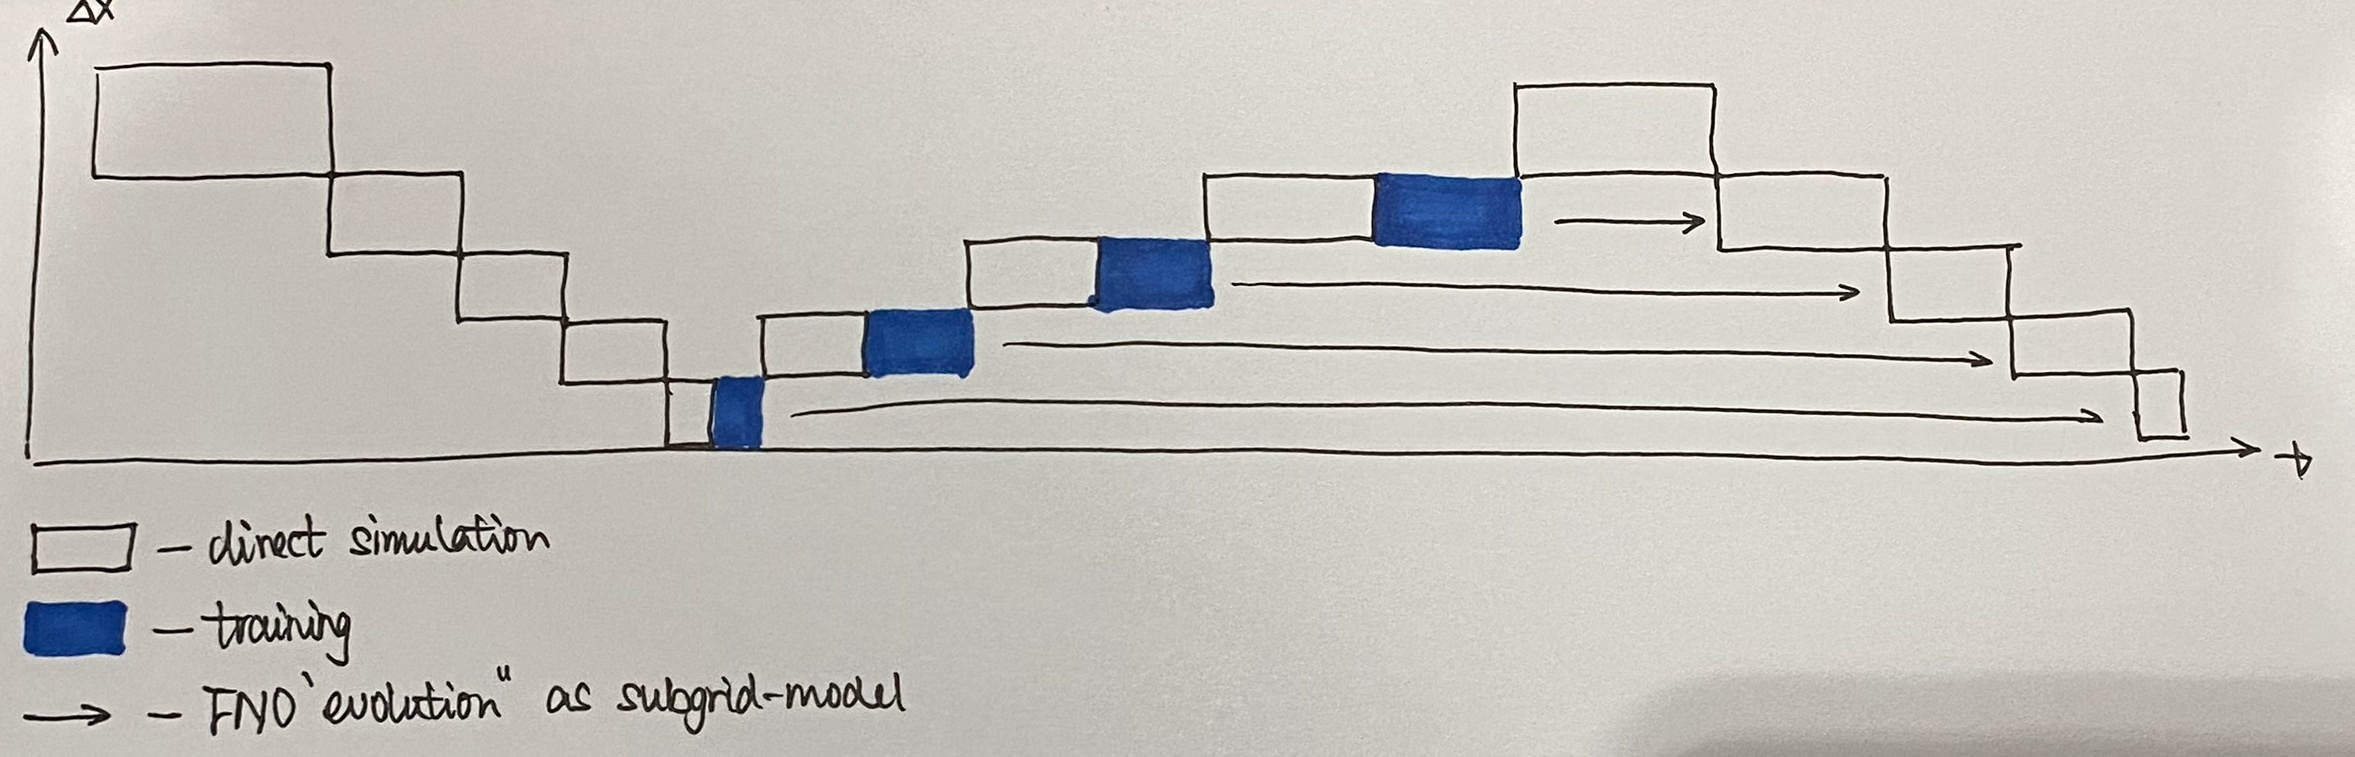
\includegraphics[width=0.8\linewidth]{figures/cyclic-zoom-fno.png}
%     \caption{
%     The schematic spatial-temporal V-cycle diagram for direct cyclic-zoom numerical simulation and in-time training with FNO. During zoom-out, the downsampled simulation data is used for training FNO, and the inner boundary condition with one higher level is provided by the long-time roll-out of FNO accordingly.
%     } 
%     \label{fig:cyclic-zoom-fno}
% \end{figure*}

\section{Diagnostics}

\subsection{Hydrodynamics}

\subsection{MHD}

\subsection{GRMHD}
For consistency, we apply the diagnostics same as the previous GRMHD simulation \cite{Guo:2025sjb}. The relevant diagnostics include mass flux, magnetic field flux, energy flux, radial momentum flux, and angular momentum flux:
\begin{align}
    \dot{M}&\equiv-\int_S \rho u^r\sqrt{-g}\,d \Omega,\\
    \Phi_\mathrm{BH}&\equiv \sqrt{\pi} \int_S |B^r|\sqrt{-g}\,d\Omega,\\
    \dot{E}&\equiv \int_S \tensor{T}{^r_t}\sqrt{-g}\,d\Omega,\\
    \dot{p_r}&\equiv \int_S \tensor{T}{^r_r}\sqrt{-g}\,d\Omega,\\
    \dot{L}&\equiv \int_S \tensor{T}{^r_\phi}\sqrt{-g}\,d\Omega,
\end{align}
where $S$ is the area, $\tensor{T}{^r_t}=(\rho+u+p+b^2)u^{r}u_{t}-\tensor{b}{^r}\tensor{b}{_t}$, and $\tensor{T}{^r_\phi}=(\rho+u+p+b^2)u^{r}u_{\phi}-\tensor{b}{^r}\tensor{b}{_\phi}$.
Sometimes it is useful to separate the mass flux into inflow and outflow:
\begin{equation}
    \dot{M}=\underbrace{-\int_{u^r<0}\rho u^r\sqrt{-g}\,d \Omega}_{\dot{M}_\mathrm{in}}-\underbrace{\int_{u^r>0}\rho u^r\sqrt{-g}\,d \Omega}_{\dot{M}_\mathrm{out}}.
\end{equation}
The dimensionless magnetic flux parameter is defined by
\begin{equation}
    \phi_\mathrm{BH}\equiv\frac{\Phi_\mathrm{BH}}{\sqrt{\dot{M}}}.
\end{equation}
The energy flux $\dot{E}$ includes the flux of rest-mass energy, so the ``feedback'' energy flux is $\dot{M}-\dot{E}$. The efficiency of feedback can thus be defined by
\begin{equation}
    \eta\equiv \frac{\dot{M}-\dot{E}}{\dot{M}}.
\end{equation}
The efficiency is positive (negative) when energy is transported outward (inward). We can further separate the feedback power into the hydrodynamic part and the electromagnetic (EM) part
\begin{align}
    &\dot{E}_\mathrm{hydro}=-\int_S \left[(\rho+u+p)u^{r}u_{t}+\rho u^r\right]\sqrt{-g}\,d\Omega, \\
    &\dot{E}_\mathrm{EM}=-\int_S \left(b^2u^{r}u_{t}-\tensor{b}{^r}\tensor{b}{_t}\right)\sqrt{-g}\,d\Omega,
\end{align}

\section{Problem Setups and Datasets}
\label{sec:setup}

\subsection{Newtonian MHD from large-scale zoom-in}

\begin{itemize}
    \item floor and cap
    \item output frequency
    \item downsampled size/resolution
\end{itemize}

\subsection{GRMHD}
The initial condition is a cloud of gas with constant mass density $\rho=\rho_0$ and constant angular momentum. We cho



% \subsection{Method-Differential Programming-1: Boundary Condition}
% \hyw{directly use the trained dataset as the boundary condition}

% \subsection{Method-Differential Programming-2: Live-Training}
% \hyw{Device to Host transfer is needed, output can be downsampled and meshblock-wise outputed}


\section{Results}
\label{sec:results}



\section{Discussion and Conclusion}
\label{sec:conclusion}

\hywcom{Conclusions.}
In this work, we present a method combining neural operator and direct numerical simulations for accretion and feedback problem, in both magnetohydrodynamic and general relativistic magnetohydrodynamic simulations.

We demonstrate the validity of the method by training on MHD and GRMHD simulations of magnetized Bondi accretion onto a central black hole.


(1) 

(2)

(3)

* begin 

% Neural operators are machine learning techniques capable of learning solutions to ODE networks, such as the
% network of rate equations present in Grackle. We lay
% out a method for training these models, primarily based
% on the implementation of Branca & Pallottini (2024),
% while also introducing three variant models (which we
% refer to as Wide, Deep and WideDeep). 

% We select initial
% conditions to span a wide range of densities and energies based on the densities and energies of a cosmological
% simulation, in order to train on typical values present in
% these simulations.

% We demonstrate that our ML models are able to match
% Grackle to an excellent degree of accuracy (see Figure
% 5), and provide a computational speedup of up to a factor
% of 8 for certain density/energy ranges. Our relative errors between the ML result and the results from Grackle
% average in the range of 10−3
% , while Branca & Pallottini
% (2024) find relative errors around 10−2
% . However, they
% note an approximate speedup of 128, much greater than
% our results. Their comparison is however against Krome
% (Grassi et al. 2014), with radiation effects taken into account. This increases the number of chemical reactions,
% increasing the complexity of the chemical model. Our
% simpler chemical network takes fewer computations until
% completion, making Grackle in this configuration faster
% than the network used by Branca & Pallottini (2024).
% This increase in model complexity makes a direct comparison of the speedup challenging, and may also drive
% the difference in relative error. Nonetheless, our main
% results agree with those of Branca & Pallottini (2024) in
% that we both find excellent agreement between the ML
% approach and the direct chemistry solver for the one zone
% test and we both clearly show significant computational
% gains.
% In terms of model variants we find that after training, the fiducial model performs well, with a typical cell
% having less than 0.6 dex error over the entire time range
% considered for the one-zone tests considered, however this
% may rise to over 1.5 dex for cells with higher variance.
% However, the Wide model appears to have the best overall
% performance, outperforming the fiducial model in terms
% of both speed and accuracy. In comparison the Deep and
% WideDeep models show larger relative errors (compared
% to Grackle), this may be explained by the amount of
% training, with the deeper models requiring more training
% for equal performance.
% Overall, while these results show that DeepONet has
% the potential to work with cosmological simulations, it
% is still far from being able to fully replace the chemical
% network currently in place in many cosmological simulations. The reliability of these ML models to predict
% in lockstep with the hydrodynamical evolution of such a
% simulation is currently not at the level required for practical use. While for an individual time step the predictions are excellent, small differences expand rapidly with
% repeated iterations - quickly breaking numerical stability
% and accuracy.
% Another future challenge is the inclusion of GPU hardware in the cosmological simulation codes. The ML models laid out in this work perform best on GPU hardware,
% but many simulation codes exclusively use CPU hardware, limiting the potential speedup of ML methods.
% The training of ML models also benefits from GPU hardware, allowing larger networks to train faster on larger
% data sets, improving accuracy and performance. A full
% integration of ML methods into cosmological hydrodynamics simulations has great potential, but will have to
% overcome these challenges.

* end

This is aimed to motivate the future development of machine-learning-based subgrid models in galactic and cosmological simulations, capturing both the statistically averaged mass and energy feedback information and the variability simultaneously.

\hywcom{Future Prospective.}
The method presented in this paper is a first step (two-level version) towards a multi-level cyclic-zoom/multi-zone neural operator framework for simulations around a central accretor.

\section{Acknowledgement}
The authors are grateful for discussions with Philip Hopkins, Yoonsoo Kim, Wenrui Xu, and Hengrui Zhu.
HYW thanks Minghao Guo for discussions on a closely related project.
ERM and HYW acknowledge support from the National Science Foundation through award NSF-AST2508940.
Part of the simulations were performed on DOE OLCF Summit under allocation AST198.
This research used resources of the Oak Ridge Leadership Computing Facility at the Oak Ridge National Laboratory, which is supported by the Office of Science of the U.S. Department of Energy under Contract No. DE-AC05-00OR22725. 
Part of this project was completed during the Caltech relativistic astrophysics summer school, which was supported by the National Science Foundation. 



\clearpage

\appendix
\onecolumngrid

\begin{figure}
    \centering
    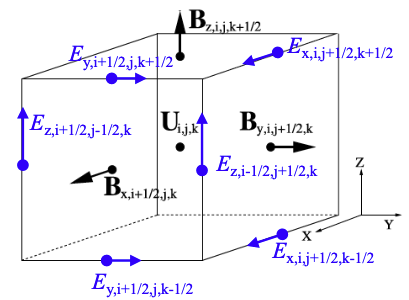
\includegraphics[width=0.3\linewidth]{figures/ct.png}
    \caption{
    Positions of hydrodynamic variables, magnetic fields, and electric fields. The hydrodynamic variables are at the body-center of each cell, while the electric fields and magnetic fields are at the face-centers and edge-centers.
    } 
    \label{fig:ct}
\end{figure}

\begin{figure}
    \centering
    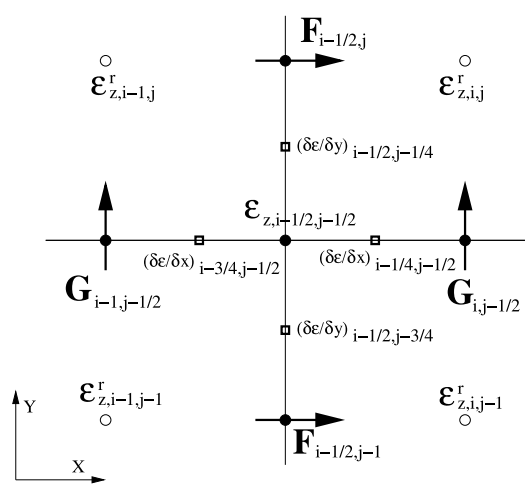
\includegraphics[width=0.4\linewidth]{figures/ct-2.png}
    \caption{
    \hywcom{Adopting from Athena method paper-remake later}
    The schematic diagram of the x-y slice, in which shows the cell-centered reference state of EMF $E^r_z$, cell-cornered EMF $E_z$ used for recovering the area-averaged magnetic field, and the fluxes of conserved variables in the x and y directions.
    } 
    \label{fig:ct-2}
\end{figure}

\section{Constraint Transport on the Boundary: NO as Riemann Solver }

\subsection{Review: Divergence-Free Magnetic Field and Constraint Transport}
The magnetic fields are evolved via Stoke's law:
\begin{equation}
\frac{\partial}{\partial t} \int_S \boldsymbol{B} \cdot d \boldsymbol{S}=-\int_L \boldsymbol{E} \cdot d \boldsymbol{l} \,,
\end{equation}
in the differential form : 
\begin{equation}
\frac{\partial \boldsymbol{B}}{\partial t}+\nabla \times \boldsymbol{E} =0 \,,
\end{equation}
where the electric field (electromotive force [EMF]) $\boldsymbol{E}=-\boldsymbol{v}\times \boldsymbol{B}$ in ideal MHD. 


Constraint transport (CT) algorithm update the area-averaged magnetic fields using the line-averaged EMF at cell corners. First, we can separately define the face-centered, area-averaged magnetic field $\left(B_x\right)_{i+1 / 2, j, k}$ and the edge-centered, line-averaged EMF $\left(E_x\right)_{i, j+1 / 2, k-1 / 2}$ as follow (taking $x$-component as an example): 
\begin{align}
&\left(B_x\right)_{i+1 / 2, j, k} =\frac{1}{\Delta y \Delta z} \int_S B_x(y, z) d y d z\, , \\
&\left(E_x\right)_{i, j+1 / 2, k-1 / 2} =\frac{1}{\Delta x \Delta t} \int E_x(x) d x d t\, ,
\end{align}



The magnetic field at the $n+1$ timestep is updated using the electro-magnetic forces accordingly
\begin{equation}
B_{x, i+1 / 2, j, k}^{n+1}=B_{x, i+1 / 2, j, k}^n-\frac{\Delta t}{\Delta y}\left(E_{z, i-1 / 2, j+1 / 2, k}^{n+1 / 2}-E_{z, i-1 / 2, j-1 / 2, k}^{n+1 / 2}\right)+\frac{\Delta t}{\Delta z}\left(E_{y, i-1 / 2, j, k+1 / 2}^{n+1 / 2}-E_{z, i-1 / 2, j, k-1 / 2}^{n+1 / 2}\right)
\end{equation}
Then the divergence of magnetic field $\nabla\cdot \boldsymbol{B}$ is preserved to machine accuracy
\begin{equation}
\nabla \cdot \boldsymbol{B}  =\frac{B_{x, i+1 / 2, j, k}-B_{x, i-1 / 2, j, k}}{\Delta x} 
 +\frac{B_{y, i, j+1 / 2, k}-B_{x, i, j-1 / 2, k}}{\Delta y} 
 +\frac{B_{z, i, j, k+1 / 2}-B_{z, i, j, k-1 / 2}}{\Delta z}
\end{equation}

\subsection{Coupling NO with Constraint Transport}
In \texttt{Athena++/K}, it is the Riemann solver that returns area-averaged electric fields at cell faces, while the CT requires the line-averaged EMF at cell corners to update the area-averaged magnetic fields, here this is achieved by \cite{Gardiner:2005JCoPh.205..509G,Gardiner2008,Stone:2008mh}:
\begin{align}
E_{z, i-1 / 2, j-1 / 2}= 
&\frac{1}{4}\left(E_{z, i-1 / 2, j}+E_{z, i-1 / 2, j+1}+E_{z, i, j-1 / 2}+E_{z, i+1, j-1 / 2}\right) \\
&+\frac{\delta y}{8}\left[\left(\frac{\partial E_z}{\partial y}\right)_{i-1 / 2, j-1 / 4}-\left(\frac{\partial E_z}{\partial y}\right)_{i-1 / 2, j-3 / 4}\right] \\
&+\frac{\delta x}{8}\left[\left(\frac{\partial E_z}{\partial x}\right)_{i-1 / 4, j-1 / 2}-\left(\frac{\partial E_z}{\partial x}\right)_{i-3 / 4, j-1 / 2}\right] \,,  \label{eq:ct-1}
\end{align}
where the derivatived of EMF on each cell face is computed from the upwinded contact mode from the Riemann solver, i.e., suppressing the $j$ subscript,
\begin{equation}
\left(\frac{\partial E_z}{\partial y}\right)_{i-1 / 2}= 
\begin{cases}
\left(\partial E_z / \partial y\right)_{i-1}, & \text { for } v_{x, i-1 / 2}>0 \\ 
\left(\partial E_z / \partial y\right)_i, & \text { for } v_{x, i-1 / 2}<0 \\ 
\frac{1}{2}\left[\left(\frac{\partial E_z}{\partial y}\right)_{i-1}+\left(\frac{\partial E_z}{\partial y}\right)_i\right], & \text { otherwise },
\end{cases}
\end{equation}
The cell-centered derivatives of EMF are calculated from the face-centered EMF (Godunov flux) and cell-centered reference EMF $E^r_z$ (see Fig. \ref{fig:ct-2}):
\begin{equation}
\left(\frac{\partial E_z}{\partial y}\right)_{i, j-1 / 4}=2\left(\frac{E_{z, i, j}^r-E_{z, i, j-1 / 2}}{\delta y}\right), \label{eq:ct-2}
\end{equation}
For more details on how to compute the reference EMF in certain timestep \hywcom{refine the description here}, see \cite{Stone:2008mh}. 

Since the NO is trained to predict the cell-centered volume-averaged magnetic field, from Eq. \ref{eq:ct-1} and \ref{eq:ct-2}, we replace the face-centered EMF from Riemann solver with that from NO prediction (using the )



\section{Global Angular Momentum Transport}
\label{app:amt}

\subsection{Cylindrical Coordinate}

In this section we want to briefly review the equations governing the transport of total angular momentum. We do so by starting out with the ideal MHD equations in cylindrical coordinates. Denoting %$\varpi$ 
$R$ as the cylindrical radius and $z$ as the height coordinate, the conserved angular momentum density $j$\footnote{\hyw{The specific angular momentum is $l=R v_\phi$. To have the conserved angular momentum in the radial direction, one need to do the integration along both azimuthal and vertical directions $\int R d\phi \int dz \rho l=\int d\phi \int dz (R^2 \rho v_\phi)$. So the conserved angular momentum current across different cylinders (having $R$ constant) has the form of $j=R^2 \rho v_\phi$}} then given by
\begin{align}
    j = R^2 \rho v_\phi\,
\end{align}
The momentum equation then takes the form
\begin{align}
    \partial_t j + \partial_R \left( j v_R + R^2 B_R B_\phi \right) + \partial_\phi \left( {j} + R B_\phi B_\phi + R \bar{P}\right) + \partial_z \left(j v_z  + R^2 B_z B_\phi\right) - R \rho \partial_\phi \Phi_g = 0.
\end{align}
In practice, we are mainly interested in the transport of angular momentum in radius $R$ and height $z$, so we will average over the $\phi$ direction. This is appropriate for both the outer and the individual minidisks.
Defining the azimuthally averaged angular momentum density,
\begin{align}
    \left<j\right>_\phi = \int_0^{2\pi}{\rm d}\, \phi j\,
\end{align}
we obtain
\begin{align}
\partial_t \left<j\right>_\phi + \partial_R \left( \left<j v_R \right>_\phi + R^2 \left<B_R B_\phi\right>_\phi \right) + \partial_z \left(\left< j v_z \right>_\phi + R^2 \left<B_z B_\phi \right>_\phi \right) - R \left<\rho \partial_\phi \Phi_g\right>_\phi = 0.
\end{align}
the components appearing as derivatives in $\phi$ are canceled from the azimuthally periodic nature.

\subsection{Spherical Coordinate}

\subsubsection{Radial Angular Momentum Balance}

% \hyw{The angular momentum balance in the radial direction requires integrating in both azimuthal and vertical direction. The momentum equation is modified as}
% \begin{align}
% \hyw{
% \partial_t \left<j\right>_\phi + \partial_R \left( \left<j v_R \right>_\phi + R \left<B_R B_\phi\right>_\phi \right) + \partial_z \left(\left< j v_z \right>_\phi + R \left<B_z B_\phi \right>_\phi \right) - R \left<\rho \partial_\phi \Phi_g\right>_\phi = 0.}
% \end{align}

% \begin{equation*}
% \frac{\partial (\rho v)}{\partial t} +\nabla \cdot (\rho vv+\overline{P}\mathbb{I} -BB)=-\rho \nabla \Phi 
% \end{equation*}
Angular momentum flux advected along the disk can be calculated by doing the integration in the $\phi$ and z directions. For convenience, in the following we will use the notation:
\begin{align*}
\displaystyle < Q >_{\phi ,z}( R) &=\int _{0}^{2\pi } d\phi^\prime \int _{z_{\mathrm{lower}}}^{z_{\mathrm{upper}}} dz^\prime\cdot Q( R,\phi^\prime ,z^\prime) \\
< Q >_{R} &=\int_{0}^{R} dR^\prime\cdot Q(R^\prime) \\
< Q >_{t} &=\int dt^\prime\cdot Q(t^\prime)
\end{align*}
The momentum equation can be further modified as
\begin{align*}
\int dz[ \partial _{t}< j> _{\phi }]  = &-\int dz\partial _{R}< jv_{R}> _{\phi } -\int dz\partial _{z}< jv_{z}> _{\phi } \\
&-\int dz\partial _{R}\left( R^{2}< B_{R} B_{\phi }> _{\phi }\right) -\int dz\partial _{z}\left( R^{2}< B_{z} B_{\phi }> _{\phi }\right) -\int dzR< \rho \partial _{\phi } \Phi _{g}> _{\phi }\\
\partial _{t}< j> _{\phi ,z}  = &-\partial _{R}< jv_{R}> _{\phi ,z} -< jv_{z}> _{\phi } |_{z_{\mathrm{lower}}}^{z_{\mathrm{upper}}} \\
&-\partial _{R}\left( R^{2}< B_{R} B_{\phi }> _{\phi ,z}\right) -R^{2}< B_{z} B_{\phi }> _{\phi } |_{z_{\mathrm{lower}}}^{z_{\mathrm{upper}}} -R< \rho \partial _{\phi } \Phi _{g}> _{\phi ,z}
\end{align*}
We can reformulate the radial balance into a more compact form: 
\begin{equation*}
\partial _{t}\left(\frac{dJ}{dR}\right) =\frac{\partial \dot{J}_{\mathrm{adv} ,R}}{\partial R} +\frac{dT_{\mathrm{adv} ,z}}{dR} +\frac{\partial \dot{J}_{\mathrm{mag} ,R}}{\partial R} +\frac{dT_{mag,z}}{dR} +\frac{dT_{\mathrm{grav}}}{dR}
\end{equation*}
where we have defined 

\begin{equation*}
\begin{aligned}
 & ( 1) \ \mathrm{radial\ dependence\ of\ total\ angular\ mometum} & \frac{dJ}{dR} & =-< j> _{\phi ,z}\\
 & ( 2) \ \mathrm{inward\ angular\ momentum\ flux\ from\ advection} & \dot{J}_{\mathrm{adv} ,R} & =-< jv_{R}> _{\phi ,z}\\
 & ( 3) \ \mathrm{torque\ from\ vertical\ transport( wind)} & \left< \frac{dT_{\mathrm{adv} ,z}}{dR}\right> _{R} & =-\int dR^\prime < jv_{z}> _{\phi } |_{z_{\mathrm{lower}}}^{z_{\mathrm{upper}}}\\
 & ( 4) \ \mathrm{inward\ angular\ momentum\ flux\ from\ magnetic\ transport\ in\ the\ radial} & \dot{J}_{\mathrm{mag} ,R} & =-R^{2}< B_{R} B_{\phi }> _{\phi ,z}\\
 & ( 5) \ \mathrm{magnetic\ torque\ per\ unit\ radius} & \left< \frac{dT_{mag,z}}{dR}\right> _{R} & =-\int dR^\prime R^{\prime 2}< B_{z} B_{\phi }> _{\phi } |_{z_{\mathrm{lower}}}^{z_{\mathrm{upper}}}\\
 & ( 6) \ \mathrm{gravitational\ torque\ per\ unit\ radius} & \left< \frac{dT_{\mathrm{grav}}}{dR}\right> _{R} & =-\int dR^\prime R^\prime < \rho \partial _{\phi } \Phi _{g}> _{\phi ,z}
\end{aligned}
\end{equation*}
After we do the time averaging of the above equation and assume a steady state of accretion $\displaystyle ( \partial _{t} =0)$, the accretion disk reaches a steady state. 
\begin{equation*}
\frac{d<\dot{J}>_t}{dR} =\frac{\partial }{\partial R}(< \dot{J}_{\mathrm{adv} ,R}> _{t} +< \dot{J}_{\mathrm{mag} ,R}> _{t}) +\left< \frac{dT_{\mathrm{adv} ,z}}{dR}\right> _{t} +\left< \frac{dT_{mag,z}}{dR}\right> _{t} +\left< \frac{dT_{\mathrm{grav}}}{dR}\right> _{t}
\end{equation*}
Integrating along the radial direction from the coordinate pole (which is also the location where different torque components vanishes due to $\displaystyle R\equiv 0$), we have 
\begin{equation*}
 <\dot J_{B}>_t=\dot{<J>_t}=< \dot{J}_{\mathrm{adv} ,R}> _{t} +< \dot{J}_{\mathrm{mag} ,R}> _{t} +\left< \frac{dT_{\mathrm{adv} ,z}}{dR}\right> _{R,t} +\left< \frac{dT_{mag,z}}{dR}\right> _{R,t} +\left< \frac{dT_{\mathrm{grav}}}{dR}\right> _{R,t}
\end{equation*}
where $\dot J_{B}$ is the total torque exerted directly onto the binary.

\section{Pedagogical Introduction: GRMHD}
[Valencia Formulations] The compact form of the relativistic MHD equations can be written in the conservative Valencia formulations.
\begin{equation}
    \partial_t(\sqrt{\gamma} \boldsymbol{U})+\partial_i\left(\sqrt{\gamma} \boldsymbol{F}^i\right)=\sqrt{\gamma} \boldsymbol{S}
\end{equation}
where $\boldsymbol{U}$ is the conserved variables, $\boldsymbol{F}^i$ is the fluxes, and $\boldsymbol{S}$ is the source terms.

The state vectors $\boldsymbol{U}$, flux vectors $\boldsymbol{F}^i$, and source terms $\boldsymbol{S}$ have the following form:
\begin{equation}
    \boldsymbol{U}=\left(\begin{array}{c}
    D \\
    S_j \\
    \mathscr{U} \\
    B^j
    \end{array}\right), \quad \quad \boldsymbol{F}^i=\left(\begin{array}{c}
    D \mathscr{V}^i \\
    \alpha W^i{ }_j-\beta^i S_j \\
    \alpha S^i-\beta^{i \mathscr{U}} \\
    B^j \mathscr{Y}^i-B^i \mathscr{V}^j
    \end{array}\right),
\end{equation}
\begin{equation}
    S=\left(\begin{array}{c}
    0 \\
    \frac{1}{2} \alpha W^{i k} \partial_j \gamma_{i k}+S_i \partial_j \beta^i-\mathscr{U} \partial_j \alpha \\
    \frac{1}{2} W^{i k} \beta^j \partial_j \gamma_{i k}+W_i^j \partial_j \beta^i-S^j \partial_j \alpha \\
    0
    \end{array}\right) .
\end{equation}

\begin{eqnarray}
  \label{eq:1-1}
  &&\nabla_\mu \tilde{J}^\mu = \nabla_\mu \rho u^\mu = 0\,,\\
  %
  \nonumber \\
  %
  \label{eq:1-2}
  &&\nabla_\mu T^{\mu \nu} = 0\,,
\end{eqnarray}

We can start from the covariant continuity equation \eqref{eq:1-1}, which
can be written as

\begin{align}
\nabla_\mu \left(\rho u^\mu\right) &= \frac{1}{\sqrt{-g}} \partial_\mu
\left(\sqrt{-g} \rho u^\mu\right) \notag \\ &= \frac{1}{\sqrt{-g}}
\left[\partial_t \left(\sqrt{-g} \rho u^t\right) + \partial_i
  \left(\sqrt{-g} \rho u^i\right)\right] = 0\,, \label{eq:continuity}
\end{align}



\bibliography{cbd_ref}
\end{document}
